%!TEX root = project.tex

\chapter*{About this project}
% assuming past tense as this report is talking about the completed project
\paragraph{Abstract}
%A brief description of what the project is, in about two-hundred and fifty words.

% leave technical jargon out of it
This project sets out to create a food ordering system for a local company. 
The systems primary components are a mobile application that the user interacts with and a web application that the staff interact with.

The need for such a system stems from two problems, firstly the issue of rush hour times during business hours where there is a vast number of customers to service, and secondly to bring more presence and promotion to the business, as they are finding it hard to reach out to their current customer base and would be customers.

% Mobile app
We aim to solve the first problem by having a system in which customers can pre-order sandwiches and other products via a mobile application.
Users will be able to top up their account, order products, pick a collection time, and view their balance, products and past order history.

The second problem will be solved by implementing push notifications into the application so that the company can let customers know about menus, events and various other updates. Another way to increase promotion and presence is by having various information about the company on the application; for instance: opening times, contact details and general information. 

% web app
All of the information on the web application can be updated; this includes the menus, opening times, user and staff details, and much more. 
This information is reflected in the web application.
Interactions from within the mobile application including: topping up, logging in, registration and ordering go through the web application.

% conclusion
We plan to create a cohesive, thoughtfully designed, robust system that solves these two problems.
\pagebreak


\paragraph{Authors}
%Explain here who the authors are.
This project was created by two fourth year software development students: Ronan Connolly \& Vladislav Marisevs, as part of our Bachelors of Science honours degree in Software Development.
\\

Ronan was in charge of creating all aspects of the user facing mobile app. 
Vladislav was in charge of creating all aspects of the staff facing web app.
\\

We spent most of our shared time coming up with the overall architecture we would implement, and an interface to be used between mobile and web app for transfer of data.
\pagebreak

\paragraph{Acknowledgements}
We would like to acknowledge and thank our supervisor Dr John Healy for all the time and effort he has put into helping us throughout this project, he gave us a good structure and set milestones for us in order to keep on top of things.
\\

We'd also like to thank the GMIT Catering Company staff for the time spent meeting with us in order to continuously improve and adapt the project.

\chapter{Introduction}	% 3-5 pages
%% CONTEXT
% basic idea
We set out to create a food ordering system for the GMIT Catering Company (known henceforth as the company).
The basic structure is a mobile application (henceforth known as mobile app) for the Android and iOS systems that the user interacts with, and a server (henceforth known as web app) that the staff can log into in order to view transactions, user details and to update the mobile app.

% reason #1
The reason such a system is needed is that queues during peak times tend to be enormous and currently it's hard to service all the customers.

% reason #2
Another reason is to encourage customers to get into a habit of repeat ordering, if it is an easy process then it should increase purchases.

% reason #3
Lastly, the company wants to increase presence and promotion in the college, in order to achieve this end we have implemented push notifications where staff can send a notification to all users. On top of this the mobile application itself serves as a promotional device, containing details of various aspects of the company.
\\

%% OBJECTIVES
% actual system:
In order to develop this system we required to connect different platforms together and let them communicate. We were using Ionic Framework for creating cross mobile application that would talk to Zend Framework 2 which will act as administration website and API (Application Programming Interface) for controlling data transfer between MySQL database and mobile program.
\\

% mobile app features
The components contained within the mobile app include pages for login, registration, about the company and user details There is also a way to top up and order sandwiches.
A huge emphasis is put on design for this project, using the companies colour theme and creating a nice icon.
% tech
This mobile app was created using the Ionic Framework which is programmed primarily using the AngularJS framework.
% Ionic part:
It's a cross platform mobile application that will authenticate users using their credentials. This option will allow us to create an account wallet, identify a person and their order history. The mobile app design uses native phone features and user interface components to let user operate without any special training.
\\

% web app features
The components contained within the web app include many pages such as the login system, orders, stock, user details, vouchers(for adding credit to your account), settings(collection and opening times) and accounts(staff) pages.
% Zend part:
This web app is a administration website which allows user to configure and manage the whole system. Users can change opening, closing and food collection times. In order to access these settings users should authenticate him self and then will be able to nominate new administration members. This website also allows to view list of orders, customers and track their history.  
%Some of these routes acts as connections that informs mobile application about changes or receives 
\\

%tech
This web app was created in PHP using Zend Framework 2.
% reflection in app
Most of the information on the web app is reflected on the mobile app.

% connect the apps
The two applications talk to each other via JSON over HTTP Get and Post requests. 

% conclusion
We set out to create a well thought out, carefully designed, robust food ordering system using modern technologies.
This project could be extended in the future to be used 
\\

% mention agile
We used an agile structure where we had certain components we needed complete by specific dates.
% mention meetings
We had various meetings each month with our supervisor and several members of the company.

%% CHAPTER SUMMARIES
\section{Chapter Summaries}
Here is a summary of all the chapters in this project report.

\subsection*{Context}
Here we talk about how the project came about, what the initial ideas, goals and objectives were.
We'll also talk about the main components of our project, how we chose them, the alternatives we tried out and a basic overview of the usage of our food ordering system.

\subsection*{Methodology}
An insight into how we began the project, the research, our technology and design choices, our thought process and how we went about allocating tasks and organising meetings.

We'll also talk about the objectives we set out to accomplish and how we went about completing them.

\subsection*{Technology Review}
Here we talk about all the technologies that we have mentioned in this report and any others that we may have used in completing the project.

\subsection*{System Design}
An overview of the project architecture, including lots of diagrams and screen shots.

\subsection*{System Evaluation}
An evaluation of our various project components, including how we tested our system for robustness and performance.
We talk about the outcomes that were achieved in relation to what are goals were, how far we strayed from our goals and some issues we came up against.
Any limitations or opportunities we encountered in our approach and in the technologies we chose.

\subsection*{Conclusion}
A broad overview of our development work-flow, from our thought processes, meetings, technology choices to our issues,problems and perceptions of the project as a whole.
We'll touch on our overall experience and what we would have done differently.

% - List the resources URL(GitHub address for the project and provide a brief list of the main elements at the URL)
\section{GitHub Links}
The web and mobile app repositories are private so you must ask to be added as a collaborator in order to view them.
Each section below has a clickable heading and contains a link to the respective GitHub repository.

\subsection*{\href{https://github.com/GMIT-Catering}{GMIT Catering Organisation}}
This GitHub organisation was created to host all repositories related to this project \cite{github_org}.
These projects will be maintained here or forked here on completion.

\subsection*{\href{http://gmit-catering.github.io/final-year-project-template/}{Gist ReadMe}}
This contains basic instructions for using each component of the project \cite{gh_gist_readme}.

\subsection*{\href{https://github.com/VMarisevs/CanteenOrderSystem}{Web App}}
The food ordering web app \cite{gh_web_app}.

\subsection*{\href{https://github.com/RonanC/gmit-catering}{Mobile App}}
The Ionic mobile application \cite{gh_mobile_app}.

\subsection*{\href{https://github.com/RonanC/gmit-catering-test-server}{Test Server}}
The test server that we used initially to test the mobile app \cite{gh_test_server}.
This received requests and sent back mock data that imitated the real server.

\subsection*{\href{https://github.com/RonanC/gmitcat-push}{Push Web App}}
This web application is using the MEAN stack technologies \cite{gh_push_webapp}.
It is hosted on Heroku and is used to save user details.
Administrators can log in and send push notification messages to registered users.

\subsection*{Project Report}
The project report that you are currently reading \cite{gh_project_report}.

\chapter{Context}	% 3-5 pages

\begin{itemize}
\item Our project consists of creating a food ordering system for the GMIT Catering Company.
\item Our basic objectives were to create a mobile and web application to deal with the above item.
\end{itemize}

% - Briefly list each chapter/section and provide 1-2 line description of what each section contains
Below we will:
\begin{itemize}
\item explain the various components of our project.
\end{itemize}

\section{System Administration and Management Web Application}
% Todo: Vlad
I decided to do this because of that, etc
PHP is great but maybe a Java web server would have being better, easier to modify, I already know Java.
SQL is hard to change over time, maybe implementing a NoSQL database would have been good...

\section{Mobile App}
The mobile application is created using bleeding edge technologies such as the Ionic framework, which utilizes the AngularMVW framework, which in turn is programmed using JavaScript. HTML and CSS were also heavily utilized.
\\

Initially I had no idea about JavaScript, web development or cross platform development. I spent much time studying JavaScript, Angular, Ionic, and the MEAN Stack (MongoDB, ExpressJS, AngularJS, and NodeJS). I then spent a lot fo time trying out various cross platform development frameworks.
\\

I will speak more in detail about these technologies in the technology review chapter.
\\

Some of the features of the mobile application are:
\begin{itemize}
\item Login
\item Sign-up
\item Password Reset
\item Food Ordering
\item About Information
\item Account Information
\item Password change
\item User History
\item Topping up
\end{itemize}
I will go through these features in detail in the system design chapter.

\subsection{Cross Platform Frameworks}
I first tried out Cordova \cite{cordova}, which I found had the capabilities to do pretty much anything, but the community and framework is very sparse, it's hard to get anything up \& running, and the styling's are horrid.
\\

Next I tried out JQueryMobile \cite{jquery_mobile} which had better styling but again I came across many issues.
\\

Finally I came across the Ionic Framework which uses Cordova underneath. This framework has a huge community of developers, it has the support of Google, Microsoft and many other large companies. They closely work with the Angular team at Google and the TypeScript team at Microsoft. 
They have a 24/7 group chat system set up with various sub rooms. 
They have amazing documentation, regular blog posts, quick response to questions on the blog, forums and chat. 
With Ionic you get:
\begin{itemize}
\item All the capabilities of Cordova, which allows you to access the Mobiles native APIs easily
\item A slick native UI experience. The app changes design depending on the platform it's running on
\item Extensive tooling. Starting an app, templates, app store image creation, logo creator, etc
\item Rapid development cycle, there are constant updates (which can cause issues, but is usually great)
\end{itemize}
\cite{ionic}

\subsection{Tooling}
Once I decided on using the Ionic framework I spent my time completing various JavaScript, Angular and Ionic tutorials. This was a steep learning curve as there is so much tooling for all the JavaScript frameworks.
I installed NodeJS in order to use NPM (Node Package Manager) in order install Ionic. 

Then Ionic came with it's own tools for various tasks, including SASS for programmatic CSS, Bower (Like NPM or Maven) for adding in new components, Grunt for running tasks (like Ant) and some others like Gulp (similar again to NPM).

Each of these tools takes time to learn. I read documentation and completed at least one tutorial for each.

\section{Push Server}
In order to facilitate push notifications I needed to get their device token and save it in a database.
I created a controller in the mobile application, once the app starts it gets the device token along with some other information and sends it to the push server.

The push server is always listening for incoming requests, once it receives one it evaluates it, adds a timestamp and saves the user object (JSON) to a CouchDB server (Using IBM's Cloudant Web Server).

The push server is a MEAN Stack, Yeoman scafolded project that uses NodeJS as the environment, Express as the Web Framework and Angular as the MVC (Model View Controller) framework in order to build the web application.
\linebreak

The reasons we chose to have the push notification server separate is that:
\begin{itemize}
\item We did not realise we needed to save the device tokens initially and to implement this new table into the SQL schema is a big effort
\item We wanted to try out a MEAN Stack application
\item We felt there was no big dissadvantage on having the push server seperate
\item The mobile app is so tightly integrated with the push server (everything is written in JavaScript), that it made creating the web application extremely simple
\item The GMIT Catering company may assign the task of push notifications to somebody that they do not wish to have access to the food ordering system, such as a social media expert. 
\end{itemize}

Users can:
\begin{itemize}
\item Login/Logout via username and password
\item View how many devices are registered for push notifications
\item View previously sent push notifications
\item Send new push notifications, and see if they were sent successfully.
\end{itemize}


\chapter{Methodology}	% 1-2 pages
% Describe the way you went about your project:
\begin{comment}
\begin{itemize}
	\item We used an Agile / incremental and iterative approach to development. 
	\item There were plenty of meeting and planning with our supervisor and the companies manager.
	\item We did user testing on the app, and constantly made sure all the routes were working.
	\item We designed a RESTful style route interface. This let us work on our own components without the web and mobile app waiting for each other.
	\item We used GitHub during the development process, tracking tasks via the Github Issue tracker.
	\item We tested out various technologies at each step of the way and discussed why we were choosing each one.
\end{itemize}
\end{comment}
When we began this project we knew we had to split it up into sections and allocate parts to one another.  
Since Ronan had worked on many mobile applications before and Vlad had created various web applications in conjunction with large databases we decided Ronan would take on the mobile side and Vlad the web app \& database.
\\

We have already spoken in the Introduction why we chose the technologies we chose so here we will focus on our implementation of these technologies.

\section{Direction}
%How we went about our project
We decided that we wanted to go through this project in a modern way so we looked into the \textit{"Manifesto for Agile Software Development"} \cite{manifesto_for_agile}:
\begin{figure}[H] 
	\center{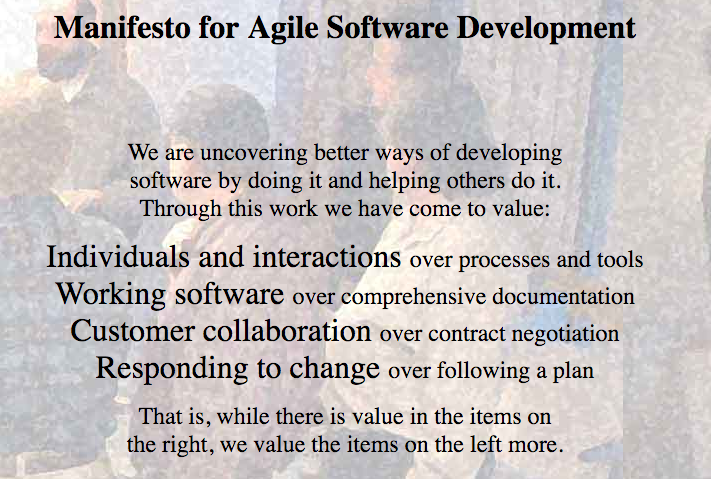
\includegraphics[width=1.0\linewidth]{img/manifesto_for_agile}}
	\caption{Manifesto for Agile Software Development}
	\label{fig:speciation}
\end{figure}
With these ideas behind us (and some more taken from SCRUM and RAD) we worked to:
\begin{itemize}
\item Have regular meetings with our client
\item Constantly take feedback on board
\item Change designs throughout development where possible
\item Break down tasks into their constituents and work through them
\end{itemize}

We used the GitHub issue tracker to work through tasks, flag bugs and add enhancement requests.
We found that the regular meetings and feedback were great for tweaking design but it held us back in many respects.
There were times when we needed to overhaul the design that took much time, especially when it involved changing the database scheme (SQL does not like this).

\subsection{Interface}
Due the fact that the mobile app relied on the server which would not be complete for some time, we needed to come up with a common interface we could both program towards.
This idea was inspired by Edsgar Dijkstra:
\begin{quote}
	% \blindtext
	\itshape He worked closely with Bram J. Loopstra and Carel S. Scholten, who had been hired to build a computer. Their mode of interaction remains a model of disciplined engineering: They would first decide upon the interface between the hardware and the software, by writing a programming manual. Then the hardware designers would have to be faithful to their part of the contract, while Dijkstra, the programmer, would write software for the nonexistent machine. Two of the lessons he learned from this experience were the importance of clear documentation, and that program debugging can be largely avoided through careful design.
	\hfill 
	\\
	- The University of Texas at Austin - The General Faculty \cite{dijkstra_interface}
	% \par
	% \begingroup
	% \leftskip4em
	% \rightskip\leftskip
	% \blindtext
	% \par
	% \endgroup
	% \blindtext
\end{quote}

We decided to create a RESTful API on your web server, to which the mobile application could query.
In order to test the mobile application in the mean time, we created a test server that would receive a request and return mock data.
We could then switch between the real and test server with one line of code change.
This also helped us find bugs, if the test server worked and the real server did not, then we knew there was an error on the real server.
This test server was written with the MEAN stack of technologies (except without MongoDB).
\\

MEAN:
\begin{itemize}
\item MongoDB
\item ExpressJS
\item AngularJS
\item NodeJS
\end{itemize}

The reason we chose this is that for RAD (Rapid Application Development) the MEAN stack is very easy to use.
Especially since the Ionic framework is already using AngularJS and shares many of the same tools including the NPM (Node Package Manager).
\\
\pagebreak
Here is a piece of code from the test server.
This code is for logging in:
\begin{minted}[%
breaklines,
mathescape,
linenos,
numbersep=5pt,
frame=single,
numbersep=5pt,
xleftmargin=0pt,
]{js}
// login
app.get('/verifyuser/:customerLg/:customerPW', function(req, res){
    var result = {
        "customer_id":"11E4E6370B663F0D81B9EC9A743CC2AE",
        "customer_name":"Regina",
        "customer_surname":"Walsh",
        "customer_cash":"10.20",
        "customer_mobile":"0853243435"};

    res.contentType('application/json');
    res.send(JSON.stringify(result));
});
\end{minted}
\begin{comment}
This is for minted
[%
breaklines,
mathescape,
linenos,
numbersep=5pt,
frame=single,
numbersep=5pt,
xleftmargin=0pt,
]
\end{comment}
I hosted this test server on Heroku \cite{heroku}.
Heroku hosts projects as git projects, so you just need to add a config file and push to your heroku repository.
Once complete your project is running live in the wild.
Again this is another nudge towards RAD.

\subsection{Bleeding Edge Technologies}
We wanted to use bleeding edge technologies in our project, since this is our final year project we wanted to use it as a chance to research some novel technologies and see what is possible, while at the same time creating a robust system with a well thought out design.
\\
While cutting edge refers to the newest technology, it also infers that the technology has gone through the wars and is battle-tested (to a degree where it can be considered for review). 
\\
Bleeding edge is different in the sense that it is so new, that we don't even know if it will be around for very long, or whether the current merit it is receiving is worthy or is caused by the hype at the time.
\\
Bleeding edge technologies are all around, especially right now within the web development community, it seems there is a new framework or API that you \textbf{must} know every other day.
\\
We chose some bleeding edge technologies that we felt would stand the test of time and make it into the \textit{cutting edge} stage.
Here is a list of some of these technologies:
\begin{itemize}
	\item AngularJS
	\item Ionic Framework
	\item NodeJs \& ExpressJS
	\item Heroku
\end{itemize}

AngularJS is owned by Google, and Microsoft have started working with them.
This is a good indication of a solid technology, along with all the statistics on it's performance and adoption.
\\
The Ionic Framework has grown to be the most popular cross platform framework.
They work closely with the AngularJS team, and they were even presenting at the Microsoft Build 2016 conference, which is interesting since Microsoft just bought Xamarin which would be considered a competitor.
\\
NodeJS and ExpressJS were used for the test server and the push web application. 
These are still in there infancy but the Node Package Manager (NPM) has in a few short years grown to be the most popular package management system out there.
\\

Here are some graphs showing the growth trend among various package managers:
\begin{figure}[H] 
	\center{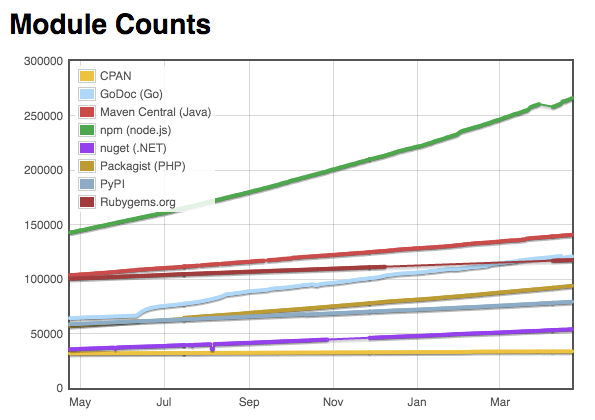
\includegraphics[width=0.75\linewidth]{img/module_counts_year}}
	\caption{Module Count Growth in the last Year }
	\label{fig:speciation}
\end{figure}
We can see here that NPM is the clear winner.
This is due to the fact that the community is so alive, connected and are really into open source software development.

\pagebreak
In this graph we can see exponential growth from NPM:
\begin{figure}[H] 
	\center{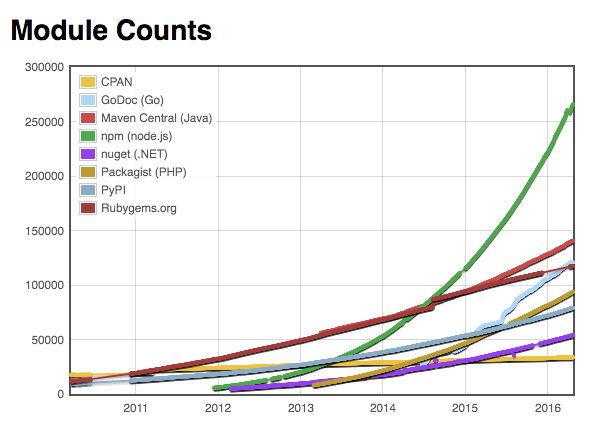
\includegraphics[width=0.75\linewidth]{img/module_counts_alltime}}
	\caption{Module Count Growth All-time }
	\label{fig:speciation}
\end{figure}

Server Providers that use the git \cite{git} technology to allow users to manage their servers are becoming increasingly more popular as time goes on.
Examples of this our companies like Heroku.
This makes it very easy to maintain, manage and utilize a RAD type of development.



\section{Agility}
% Agile / incremental and iterative approach to development. Planning, meetings.
\subsection{Agile}

\subsection{Meetings}

\subsection{Team Work}

\section{Testing}
%What about validation and testing? Junit or some other framework.
\subsection{Test Server}

\section{Source Control}
%If team based, did you use GitHub during the development process.
\subsection{GitHub}

\section{Choice}
%Selection criteria for algorithms, languages, platforms and technologies.
We already mentioned in the Context chapter about why we chose Ionic, Zend and Mean stack framework/architectures.
Here we will discuss why we chose PHP, SQL, JavaScript and JSON as our core technologies.
\subsection{PHP}
% TODO: Vlad: Why PHP?
\subsection{SQL}
% TODO: Vlad: Why SQL?
\subsection{JavaScript}

\subsection{JSON}

% TODO: Vlad: Add something in relation to the web server

\chapter{Technology Review} % 7-10 pages
% intro to tech review, bla bla bla
Here we will talk about all the technologies we used.

  \section{System Administration and Management Web Application}	% 4 pages
  After gathering all system requirements and we have done a research and based on them I decided to use PHP based framework because there is a lot of hosting companies that support this server scripting language and it has very cheap pricing.
  

    \subsection{php}
	PHP is in the market since 1995 and is one of the widely used server scripting language. It is quite powerful tool for making dynamic web pages and it is free. There are many popular websites that are written on \textbf{\textit{php}} such as Facebook, Wikipedia, Flickr, Mailchimp, Wordpress.com. PHP code can be embedded into html page. This type of structure allow to use it in various web template systems, content management systems or web frameworks. From beginning \textbf{\textit{php}} wasn't object oriented language, but in the later versions they redesigned it.

    \subsection{Zend Framework 2}
		Prototype was developed using \textbf{\textit{Zend Framework 2}}. This is an open source framework for developing Web applications and services. It was written on \textbf{\textit{php}} and it is loosely coupled architecture, which allow developer to code each component independently and designed with Model View Controller structure. \textbf{\textit{Zend Framework 2}} uses 100\% object-oriented code and utilises most of the new features of \textbf{\textit{PHP 5.3}}, namely namespaces, late static binding, lambda functions and closures.~\cite{ZendFramework-Website-About}
		
		%------------------------------------------
		\begin{wrapfigure}{r}{2.5cm}
			
\includegraphics[width=3cm]{img/zf2/zf2-logo.png}
		\end{wrapfigure} 
		%------------------------------------------
		Barry and Elhakeem~\cite{ZendFramework-Security-Model} argues that Zend Framework enables simple, rapid and agile web application development process, and it also offers AJAX support to convert XML data into JSON format and integrates the most widely used APIs and Web Services of third-party companies such as Google, Microsoft, Amazon, Flickr and Yahoo. ZF provides many options for validation such as Dojo tools it also allow to filter all inputs.
		
		%Zend Framework 2 is connected to a local MySQL relational database management system, to store the information about customers, orders and user accounts. The connection is established using ZF2 DB Adapter and Mysqli driver.
		
		%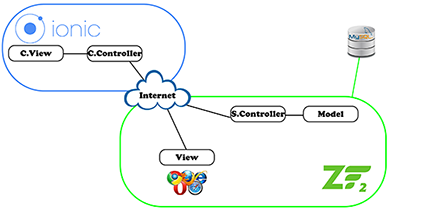
\includegraphics{img/zf2/ionic_zf2_mysql_diagram.png}
		
		Based on Hyun Jung La and Soo Dong Kim publication we can say that this project has a Balanced Model View Controller Architecture ~\cite{MVC_Architecture_for_Developing_Service-based_Mobile_Applications}. The \textbf{\textit{Zend Framework 2}} contains applications business logic or Model. And it is also responsible for validating user inputs or Server Side Controller and  Web application Views. While \textbf{\textit{Ionic}} is responsible for Client Side View and Controller (on the smartphone). In this case Mobile application uses \textbf{\textit{zf2}} Controllers to connect to \textbf{\textit{MySQL}} database.


			\subsubsection{QR code generator}
			QR codes are very popular type of two-dimensional barcode~\cite{QR_code_google}. This module was used for generating QR codes for vouchers. When voucher is printed users can scan this code and top up their balance. This module is overridden  for Zend Framework 2 and it uses Google Developers QR code generation API.~\cite{QR_code_generator}
			
			\subsubsection{DOM PDF module}
			In order to generate \textit{*.pdf} file I have used DOM PDF module for Zend Framework 2. This is most common plugin that let me to solve problems with printing remote image. It is easy to use, because it parses HTML as DOM object and generates pdf file based on that.~\cite{DOM_PDF_module}

    \subsection{MySQL}
%------------------------------------------
\begin{wrapfigure}{r}{2.5cm}
	
\includegraphics[width=3cm]{img/zf2/mysql-logo.png}
\end{wrapfigure} 
%------------------------------------------
To store information we were using \textbf{\textit{MySQL}} database management system. It's reliability is proven through the years. \textbf{\textit{MySQL}} offers complete ACID (atomic, consistent, isolated, durable) transaction support, unlimited row-level locking, distributed capability, and multi-version transaction support where readers never block writers and vice-versa. Easy manageable platform that allow a DBA to manage, troubleshoot, and control the operation of many \textbf{\textit{MySQL}} servers from a single workstation. ~\cite{MySQL_Top10_Reasons}

    \subsection{Composer}
%------------------------------------------
\begin{wrapfigure}{r}{2.5cm}
	
\includegraphics[width=3cm]{img/zf2/composer-logo.png}
\end{wrapfigure} 
%------------------------------------------
For such large distributed projects like this more often used some sort of dependency managers, that allow to force the development cycle and reuse any of already written packages. One of the most popular dependency manager for \textbf{\textit{php}} is \textbf{\textit{composer}}.
After installing it we can start using it, simply by creating \textit{composer.json} file which describes the dependencies for your project and may contain other metadata as well.~\cite{Composer_doc} 

\textbf{\textit{composer.json}} example:

\begin{minted}{json}
{
    "require": {
        "php": ">=5.5",
        "zendframework/zendframework": "~2.5",
        "zendframework/zftool": "dev-master",
    }
}
\end{minted}

As you can see, require takes a key value pairs where key maps to package names and value is version of it. We also can configure the minimal supported release or nominal version. When \textit{composer.json} is completed, we can run command that will download chosen packages and configure them in our project. To do that run this command in console:
\begin{minted}{bash}
 $ php composer.phar update
\end{minted}

    \subsection{WAMP Server}

    \subsection{Server Grove Hosting}
There is not so many hosting companies that supports Model View Controller structured \textbf{\textit{php}} websites, but the good old days when we were querying \textit{*.php} files are gone. This type of structure hides the extension and it will confuse the attacker on what sort of platform it was written.

One of most popular hosting companies in Ireland is Blacknight Solutions. For one of my portfolio websites I was using their services. At that time I was not bothered with developing my own website from the scratch and I have used \textit{Drupal} Content Management System. It is quite easy to install and setup CMS for lite blog type of website, but when it comes to connecting 2 different platforms it is no longer useful. When I developed my porfolio website on \textbf{\textit{zf2}} and tried to host it on their server I had a lot of issues with their policy. Customers don't have access to main \textit{php.ini} file which can change write properties that has to be on to use MVC structured websites. 

To solve this problems I have found \textit{Server Grove} hosting company that fully supports \textbf{\textit{Zend Framework 2}}, \textbf{\textit{Git Client}} and  \textbf{\textit{composer}}. It took me a while to move my domain name from BlackNight Solutions, but once I have it done all technical support on Server Grove is brilliant.


\pagebreak
  \section{GitHub}
\begin{wrapfigure}{r}{2.5cm}

\includegraphics[width=3cm]{img/zf2/github-logo.png}
\end{wrapfigure} 
We used GitHub \cite{github} throughout our project in order to utilize source control and keeping track of versions.
We found that it was very useful in that we could have separate repositories for the different parts of the project.
When we did work on the same repository we each had our own branch to which we would merge intermittently into the \textit{master} branch.
We also used the \textit{issue tracker} to raise any issues/bugs we noticed on each others projects, or to mention an enhancement that could be incorporated.

\begin{figure}[H] 
	\center{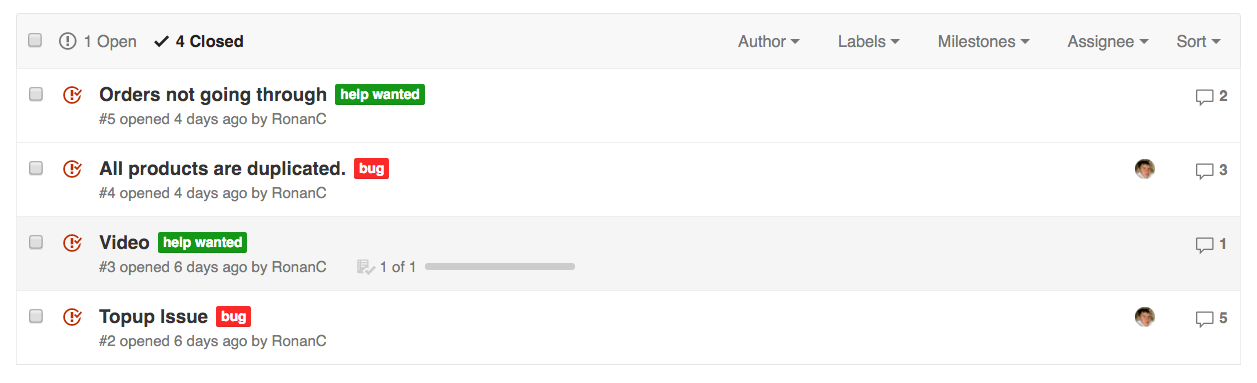
\includegraphics[width=0.75\linewidth]{img/issue_tracker}}
	\caption{Issue Tracker}
	\label{fig:speciation}
\end{figure}


We also created an organisation, which acts as an entity.
We forked all our repositories there and used it as a central hub for the overall project \cite{github_org}.
\begin{figure}[H] 
	\center{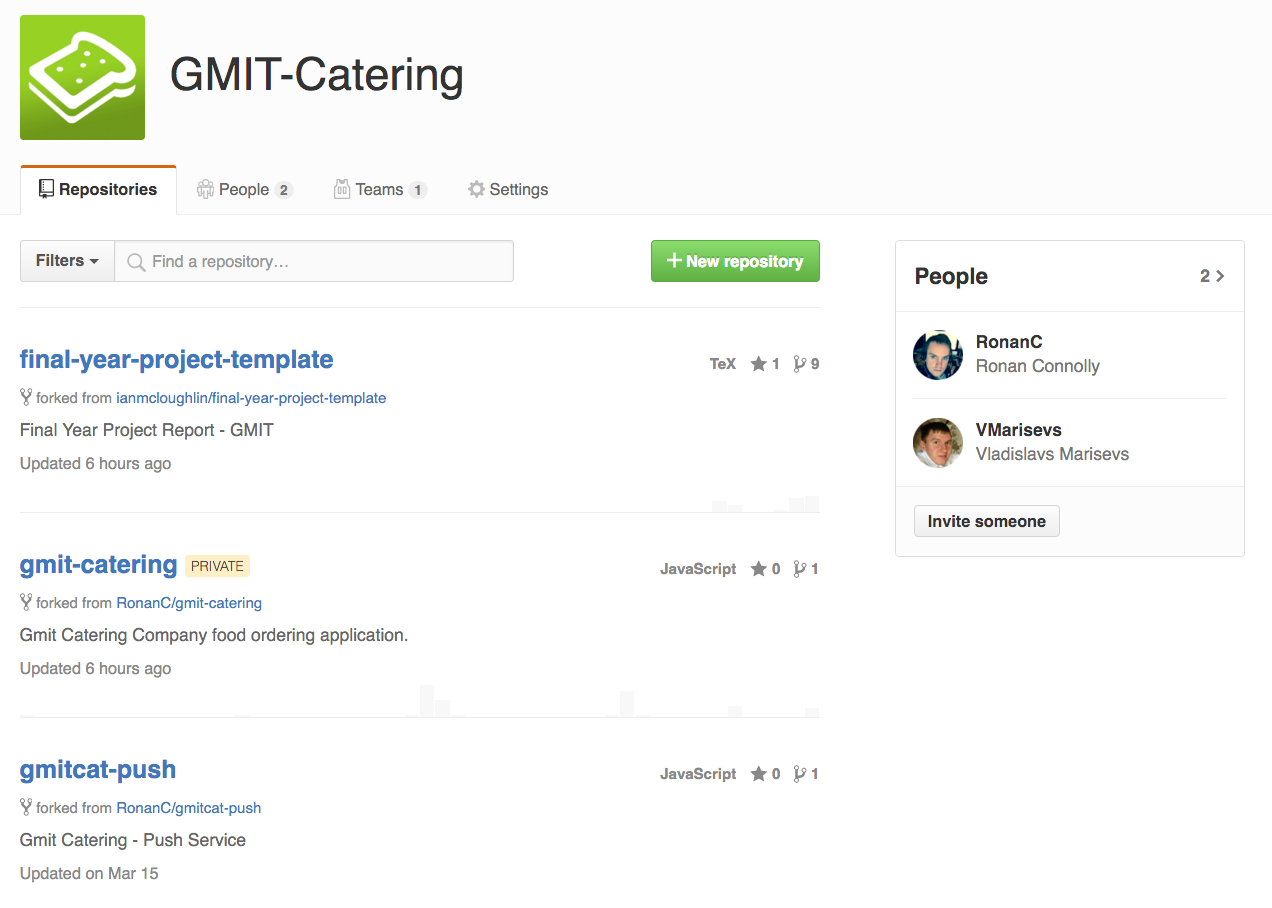
\includegraphics[width=0.75\linewidth]{img/github_org}}
	\caption{GMIT Catering GitHub Org}
	\label{fig:speciation}
\end{figure}

\pagebreak
  \section{Mobile App} % 4 pages
The technology stack I chose to use for this project is quite extensive.  
Ionic is heavily based in the JavaScript community which is known for it's enormous amount of libraries and dependencies.
It is quite a steep learning curve to get to grips with the basics, and it takes quite a while to get comfortable in the workflow.
I came across a tweet that sums up this experience:
\begin{figure}[H] 
	\center{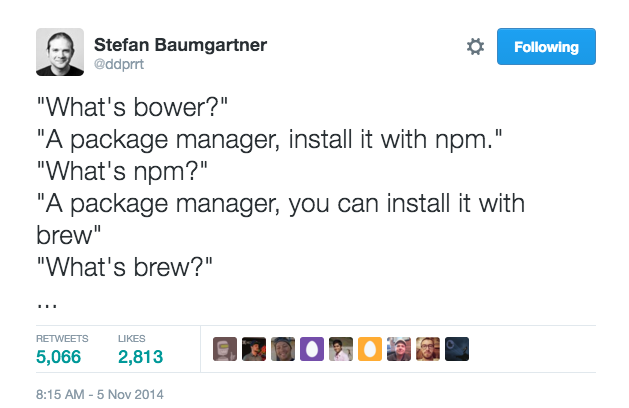
\includegraphics[width=0.8\linewidth]{img/mobile-app/js_dev_init}}
	\caption{JS Developer Learning Curve}
	\label{fig:speciation}
\end{figure}


I  done extensive research on different cross platform frameworks.
First I started with JQueryMobile and PhoneGap which had the capabilities but the community and tooling were quite scarce. 
\\ 

Xamarin was another option, It did not appeal to me as much, during my research I found many people had lots of issues with it and you still have to write some specific code for each platform.
\\ 

A lecturer of mine mentioned the Ionic framework to me and once I looked into it, it was the obvious choice.
Ionic has a huge community, extensive tooling for the majority of tasks needed and it is rapidly becoming the number one option for cross platform development.
\\

Once I had decided to take the Ionic route it meant that I was delving into the world of web development, as Ionic uses AngularJS, which is used with JavaScript, HTML, CSS and all the web development tools and work-flows.

\subsubsection{HTML/CSS}
\begin{wrapfigure}{r}{2.5cm}

\includegraphics[width=3cm]{img/mobile-app/logos/html-css.jpg}
\end{wrapfigure} 
I found that learning HTML \cite{html} and CSS \cite{css} was fine, I just needed to know enough to use Angular, which is very basic.
I had done some HTML and CSS before so I just needed to brush up on my skills.
I took the Web Development \cite{codeschool_webdev} course on Code School which helped me quickly get up to speed.
\\

HTML is great because it is a simple structure that is easy to understand.
It is just a subset of XML for websites.
\\

CSS makes is really easy to change various parts of the HTML form one place.
I used SASS (Sassy CSS), this lets you use CSS in a programmatic way (using variables).
\\

Here is a piece of SASS for the Ionic colours:
\begin{minted}[%
breaklines,
mathescape,
linenos,
numbersep=5pt,
frame=single,
numbersep=5pt,
xleftmargin=0pt,
]{css}
$light:                           #fff !default;
$stable:                          #f8f8f8 !default;
$positive:                        #5475aa !default; 
$calm:                            #11c1f3 !default;
$balanced:                        #7baa1e !default; 
$energized:                       #ffc900 !default;
$assertive:                       #840018 !default;
$royal:                           #886aea !default;
$dark:                            #444 !default;

// The path for our ionicons font files
$ionicons-font-path: "../lib/ionic/fonts" !default;

// Include all of Ionic
@import "www/lib/ionic/scss/ionic";

// custom styles
@import "scss/styles";
\end{minted}
You can also see that I am importing other style sheets.


\subsubsection{JavaScript}
\begin{wrapfigure}{r}{2.5cm}

\includegraphics[width=3cm]{img/mobile-app/logos/JS.png}
\end{wrapfigure} 
Once I had gotten myself into the basic mindset of HTML and CSS I decided to learn JavaScript.
I completed three JavaScript courses \cite{codeschool_js} on Code  School.
This gave me a great understanding of JavaScript \cite{javascript}.
\\
I found that JavaScript's event based nature took awhile to get the hang of but once understood it was very useful. 
Promises are a very important concept to understand as JS is asynchronous and tasks may not execute in order, especially blocking tasks.
This is useful as you don't need to code in concurrency, it is an inherent feature of the language.
\\
I wrote a literature review on using JavaScript for full stack development \cite{js_advantages_full_stack}, this touches on promises, the event based nature, and why JavaScript is so popular.

\subsubsection{AngularJS}
\begin{wrapfigure}{r}{2.5cm}
	
\includegraphics[width=3cm]{img/mobile-app/logos/angular.jpg}
	\centering
\end{wrapfigure}

I completed two AngularJS \cite{angular} courses on Code School. 
Then for each course I completed I done the 2/3 hour screen cast that accompanied it.
\\
The main problem I found with JavaScript is a lack of standards and structure. 
This is why I believe there are so many JS frameworks out there.
\begin{figure}[H] 
	\center{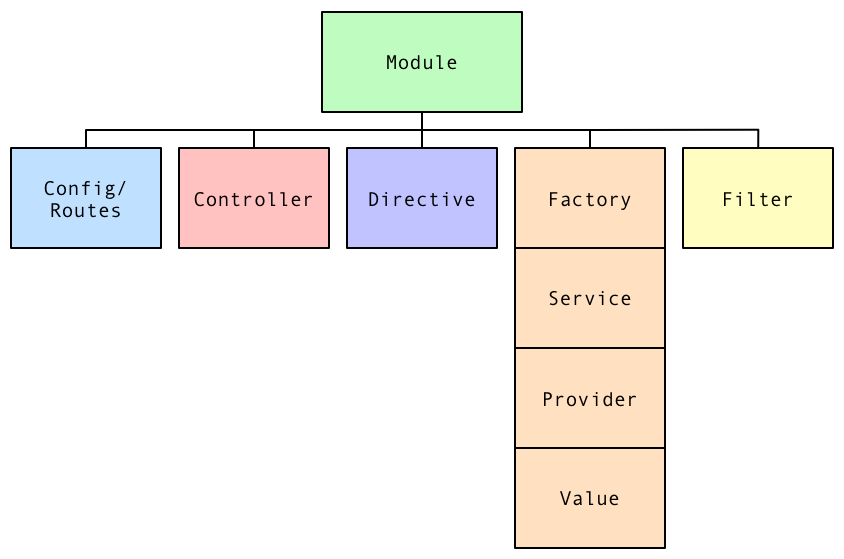
\includegraphics[width=0.75\linewidth]{img/mobile-app/angular_object_diagram.png}}
	\caption{Angular Object Diagram}
	\label{fig:speciation}
\end{figure}
A few times a year there a a new JS framework that all the web developers think is going to be the \textbf{one}.
AngularJs has risen and is now one of the top JS frameworks, partly I'm sure to do with the fact that Google is the project owner.
Competition includes Facebook's React \cite{react} and EmberJS \cite{ember}.
\\

I completed two Angular courses on Code School. 
Then for each course I completed I done the 2/3 hour screen cast that accompanied it.
\\

These helped me gain a deep understanding of controllers, services, routing and views.
Angular is based around the Model View Controller (MVC) model, where the design, data and logic are all separated.
\\
Angular is a Single Page Application (SPA). Only one page ever exists, the \textit{index.html}, then each \textit{view} is loaded into a section of this page.
Each \textit{view} has a \textit{controller} attached to it. 
The Modal contains the data which is loaded into a template that you code, this creates the view.

Two way binding is used so that as you enter information is can be seen straight away.
\begin{figure}[H] 
	\center{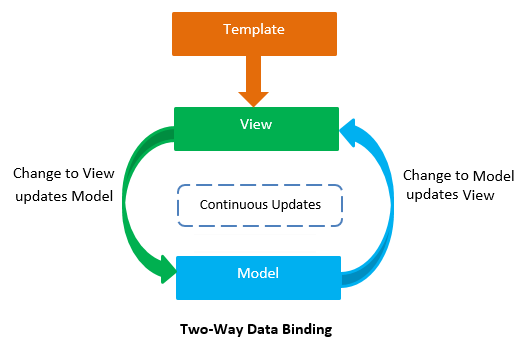
\includegraphics[width=0.75\linewidth]{img/mobile-app/two-waybinding.png}}
	\caption{Two Way Data Binding}
	\label{fig:speciation}
\end{figure}

\pagebreak
\subsection{Ionic Framework}
% talk about JS, AngularJS, CSS, HTML and Ionic.
\begin{wrapfigure}{r}{2.5cm}
	
\includegraphics[width=3cm]{img/mobile-app/logos/ionic.png}
\end{wrapfigure} 
Once I understood AngularJS I completed some Ionic tutorials on \url{EggHead.io} and \url{Thinkster.io}.

The Ionic community is really great, the forum is very engaging, questions are answered very quickly and they post to their blog regularly.
The  founders Max Lynch, Adam Bradley and Ben Sperry talk about various updates every few months on YouTube, they call this \textit{The Ionic Show} \cite{ionic_show}.
\\

To Start an Ionic application you run these commands in bash:
\begin{minted}[%
breaklines,
mathescape,
linenos,
numbersep=5pt,
frame=single,
numbersep=5pt,
xleftmargin=0pt,
]{bash}
$ ionic start myApp tabs
$ cd myApp
$ ionic platform add ios
$ ionic build ios
$ ionic emulate ios
\end{minted}
Everything is done through command line.
\\

Here is a simple controller:
\begin{minted}[%
breaklines,
mathescape,
linenos,
numbersep=5pt,
frame=single,
numbersep=5pt,
xleftmargin=0pt,
]{js}
(function() {
    'use strict';

    angular
        .module('canteen.controllers')
        .controller('AboutCtrl', about);

    about
        .$inject = ['$scope', 'Orders'];

    function about($scope, Orders) {
        $scope.opening = Orders.opening;
        $scope.closing = Orders.closing;
        $scope.times = Orders.collTimes;
    }
})();
\end{minted}
One issue I came across is that there is no definitive way to lay out structures.
This is a common issue in JavaScript, since the standards are so loose (which benefits it in order ways).
\\

The above layout follows John Papas AngularJS style guide \cite{angular_style_guide}.
John Papa works with the Microsoft team who are implementing strong typing into Angular2 (through the use of MS TypeScript).
This gives me the impression that he has a good grasp on best design practices.
\\

As you can see in the above example, I have broken up the code into its constituent components, rather then the usual nested JavaScript hierarchy.
I think it is pleasing to the eye and easy to understand.

\subsection{Heroku}

\subsection{iOS Store}

\subsection{Android Store}


\subsection{Tools}
\subsubsection{Yeoman}
\begin{wrapfigure}{r}{2.5cm}

\includegraphics[width=3cm]{img/mobile-app/logos/yeoman.png}
\end{wrapfigure} 

\subsubsection{Grunt}
\begin{wrapfigure}{r}{2.5cm}

\includegraphics[width=3cm]{img/mobile-app/logos/grunt.png}
\end{wrapfigure} 


\subsubsection{Jasmine}
\begin{wrapfigure}{r}{2.5cm}

\includegraphics[width=3cm]{img/mobile-app/logos/jasmine.png}
\end{wrapfigure} 


\subsubsection{Karma}
\begin{wrapfigure}{r}{2.5cm}

\includegraphics[width=3cm]{img/mobile-app/logos/karma.png}
\end{wrapfigure} 


\subsubsection{Bower}
\begin{wrapfigure}{r}{2.5cm}

\includegraphics[width=3cm]{img/mobile-app/logos/bower.png}
\end{wrapfigure} 


\subsubsection{NPM}
\begin{wrapfigure}{r}{2.5cm}

\includegraphics[width=3cm]{img/mobile-app/logos/npm.png}
\end{wrapfigure} 


\subsubsection{BASH}
\begin{wrapfigure}{r}{2.5cm}

\includegraphics[width=3cm]{img/mobile-app/logos/bash.jpg}
\end{wrapfigure} 

\subsection{Alternatives}
% alternatives? JQueryPhone, PhoneGap, Cordova, Xamarin
\subsubsection{Cordova}
\begin{wrapfigure}{r}{2.5cm}

\includegraphics[width=3cm]{img/mobile-app/logos/cordova.jpg}
\end{wrapfigure} 

\subsubsection{PhoneGap}
\begin{wrapfigure}{r}{2.5cm}

\includegraphics[width=3cm]{img/mobile-app/logos/PhoneGap.png}
\end{wrapfigure} 

\subsubsection{JQueryMobile}
\begin{wrapfigure}{r}{2.5cm}

\includegraphics[width=3cm]{img/mobile-app/logos/jquery-mobile.png}
\end{wrapfigure} 

\subsubsection{Xamarin}
\begin{wrapfigure}{r}{2.5cm}

\includegraphics[width=3cm]{img/mobile-app/logos/xamarin.png}
\end{wrapfigure} 

  \section{Push Server}

\subsection{CouchDB/Cloudant}
\begin{wrapfigure}{r}{2.5cm}

\includegraphics[width=3cm]{img/mobile-app/logos/cloudant.jpg}
\end{wrapfigure} 

\subsection{NodeJS}
\begin{wrapfigure}{r}{2.5cm}

\includegraphics[width=3cm]{img/mobile-app/logos/nodejs.png}
\end{wrapfigure} 

\subsection{ExpressJS}
\begin{wrapfigure}{r}{2.5cm}

\includegraphics[width=3cm]{img/mobile-app/logos/express.png}
\end{wrapfigure} 



  \section{JSON REST interface architecture}	% 1 pages
  \subsection{HTTP Requests}
  % talk about the HTTP get/post requests used via the interface from the phone and server
  \subsection{Custom API}
  % The web server has a custom API that the mobile app uses

  ~\cite{JSON_REST_interface}


\chapter{System Design}	% n-m pages
  \section{Database}
    \subsection{Purpose}

This section describes how the database that will support the system with details of the logical and physical definitions. It also provides the functional and non-functional usage of the tables, considerations and requirements.

The database design for the system is composed of definitions for db objects derived by mapping entities to tables, attributes to columns, unique identifiers to unique keys and relationships to foreign keys. 

Further in this document you will read the integration aspects of the Database with the Web Application and to understand them I want to explain some word definitions that will be used.
\\
\begin{itemize}
\item Customer is a physical person who uses smartphone application.

\item User is a physical person who operates with management website.

\item Food is entire product of this business.

\item Voucher is a printed card with unique code that allow customers to top up their account balance.
\end{itemize}
    \subsection{Procedures and Functions}
One of good reasons to use stored procedures is the added layer of security that can be placed on the database from the calling application. The risk of a attacker using the account to run a stored procedure that has been written by you is far safer than having the user account have full insert, update and delete authority on the tables directly. Another advantage to use stored procedures is the data functionality that is separated from the application making it easier to manage, document and maintain. They also improves the performance for example to make a payment I am doing just one call and DBMS can process it, which is more efficient than do complete processing on the php side.
\\

\begin{itemize}
	

\item \textbf{Verify Customer}
\\
This procedure takes two parameters login name and password, then parses it and returns the result. This procedure is used to connect Ionic application with DBMS and verify customer's credentials. If the password and login matches database returns complete details about current customer. This information can be displayed in the mobile application.

\item \textbf{Block Customer} 
\\
If system administrator sees that some user tried to enter invalid voucher id too many times, he can block this person. To keep a track of all invalid customer inputs I decided to add a basic counter, so that administrator can keep an eye on the malicious users that tries to insert voucher code permutations.

\item \textbf{Change customer's password}
\\
One of the common procedures when user is allowed to change their password if they are authorized.

\item \textbf{Insert customer}
\\
This procedure let people register their account as customer of the ordering system. To do that they have to insert their details, once that is done they can start using mobile application.

\item \textbf{Recover customer's password}
\\
In order to recover the password, user have to insert their email address and login. It will trigger the scenario of generating new temporary password for this user and will send it out to their email address. The procedure of sending emails from web application uses SMTP protocol, by default it is linked with gmail account. The settings are stored statically in configuration file \textit{*/config/autoload/email.local.php}. If login and email exists in the database it will save new password.


\item \textbf{Food insert}
\\
This procedure takes all food information, generates new identification number and returns it.


\item \textbf{Food update}
\\
In order to update the food, we are not overriding the record, but creating a new one with unique id and setting the original \textit{'active'} column to \textit{false}. This technique let us to keep track of all changes and prevent updates on the old orders.


\item \textbf{Delete Food}
\\
If user requires to remove the food, he is using this procedure. It just sets \textit{'active'} column to false and it will remove current food from list. But in case there was any orders with this food it will save a link and old details.


\item \textbf{Create order}
\\
This procedure will create an order in case it receives all valid information and returns new generated id or null which mean something is invalid.

\item \textbf{Food Order  Insert}
\\
When order is created and id returned, it starts filling it with products. 

\item \textbf{Order make payment}
\\
This procedure compares the balance on the account and if it is sufficient to make a payment it will deducts the money from user and mark the order as paid. These operations are separate to prevent incompleteness of the transaction. 

\item \textbf{Order price}
\\
This procedure calculates sum of order items and returns it.

\item \textbf{Order cancel payment}
\\
To cancel order payment we have to calculate sum of item prices and return them to customers balance.

\item \textbf{Create voucher}
\\
This function generates new voucher and places it in database.

\item \textbf{Topup customer account}
\\
Current transaction marks the voucher with customers account identification and adds money to their balance. After that this id is no longer valid for next transaction.


\end{itemize}
 
    \subsection{Tables}
    
    \subsubsection{Order System}
	    
Ionic application users table:	    
	    % Customers
	    \begin{table}[H]
	    	\centering
	    	\begin{tabular}{x{2cm}p{3cm}}
	    		\toprule \\
	    		\textbf{Column} & \textbf{Type} \\ \hline
	    		id & binary(16) \\ \hline
	    		gnumber & int(11) \\ \hline
	    		email & varchar(40) \\ \hline
	    		password & char(41) \\ \hline
	    		cash & decimal(13,2) \\ \hline
	    		active & tinyint(1) \\ \hline
	    		created & datetime \\ \hline
	    		updated & timestamp \\ \hline
	    		name & varchar(40) \\ \hline
	    		surname & varchar(40) \\ \hline
	    		address & text \\ \hline
	    		mobile & varchar(10) \\ \hline
	    		cheat & int(10) \\
	    		\bottomrule
	    	\end{tabular}
	    	\caption{Customers table}
	    	\label{table:CustomersTable}
	    \end{table}
    
    
Vouchers table:	    
	% Vouchers
	\begin{table}[H]
		\centering
		\begin{tabular}{x{2cm}p{3cm}}
			\toprule \\
			\textbf{Column} & \textbf{Type} \\ \hline
			id & varchar(16) \\ \hline
			amount & decimal(13,2) \\ \hline
			used & tinyint(1) \\ \hline
			customer & binary(16) \\ \hline
			activated & datetime \\ \hline
			created & datetime \\ \hline
			modified & timestamp \\
			\bottomrule
		\end{tabular}
		\caption{Vouchers table}
		\label{table:VouchersTable}
	\end{table}
    
Orders table:	    
	% Orders
	\begin{table}[H]
		\centering
		\begin{tabular}{x{3cm}p{3cm}}
			\toprule \\
			\textbf{Column} & \textbf{Type} \\ \hline
			id & varchar(16) \\ \hline
			customer & binary(16) \\ \hline
			comments & medium text \\ \hline
			paid & tinyint(1) \\ \hline
			collectionTime & time \\ \hline
			collectionDate & date \\ \hline
			created & datetime \\ \hline
			modified & timestamp \\
			\bottomrule
		\end{tabular}
		\caption{Orders table}
		\label{table:OrdersTable}
	\end{table}    
    
Food table:	    
	% Food
	\begin{table}[H]
		\centering
		\begin{tabular}{x{2cm}p{4cm}}
			\toprule \\
			\textbf{Column} & \textbf{Type} \\ \hline
			id & bigint(20) \\ \hline
			name & varchar(40) \\ \hline
			description & medium text \\ \hline
			price & decimal(13,2) \\ \hline
			type & enum('drink', 'roll', 'crisps', 'deal', 'misc') \\ \hline
			picture & varchar(128) \\ \hline
			active & tinyint(1) \\ \hline
			created & datetime \\ \hline
			modified & timestamp \\
			\bottomrule
		\end{tabular}
		\caption{Food table}
		\label{table:FoodTable}
	\end{table}  
    
    
Food ordered table:
	% Food ordered
	\begin{table}[H]
		\centering
		\begin{tabular}{x{2cm}p{3cm}}
			\toprule \\
			\textbf{Column} & \textbf{Type} \\ \hline
			order\_id & varchar(16) \\ \hline
			food\_id & bigint(20) \\ \hline
			count & smallint(5) unsigned \\ \hline
			created & datetime \\ \hline
			modified & timestamp \\
			\bottomrule
		\end{tabular}
		\caption{Food Ordered table}
		\label{table:FoodOrderedTable}
	\end{table}  
    
    
    
    \subsubsection{Administration}
    
Web application users table:
	    % Users table
	    \begin{table}[H]
	    	\centering
	    	\begin{tabular}{x{2cm}p{3cm}}
	    		\toprule \\
	    		\textbf{Column} & \textbf{Type} \\ \hline
	    		id & unsigned int(10) \\ \hline
	    		email & varchar(100) \\ \hline
	    		password & varchar(100) \\ \hline
	    		status & enum('Y','N') \\ \hline
	    		created & datetime \\ \hline
	    		modified & timestamp \\
	    		\bottomrule
	    	\end{tabular}
	    	\caption{Users table}
	    	\label{table:UsersTable}
	    \end{table}

	
Web application resource table:
	% resource table
	\begin{table}[H]
		\centering
		\begin{tabular}{x{2cm}p{3cm}}
			\toprule \\
			\textbf{Column} & \textbf{Type} \\ \hline
			id & unsigned int(10) \\ \hline
			resource & varchar(100) \\
			\bottomrule
		\end{tabular}
		\caption{Resource table}
		\label{table:ResourceTable}
	\end{table}
	
Web application permission table:
	% permission table
	\begin{table}[H]
		\centering
		\begin{tabular}{x{2cm}p{3cm}}
			\toprule \\
			\textbf{Column} & \textbf{Type} \\ \hline
			id & unsigned int(10) \\ \hline
			permission & varchar(100) \\ \hline
			resource & unsigned int(10) \\
			\bottomrule
		\end{tabular}
		\caption{Permission table}
		\label{table:PermissionTable}
	\end{table}

Web application role table:
	% role table
	\begin{table}[H]
		\centering
		\begin{tabular}{x{2cm}p{5cm}}
			\toprule \\
			\textbf{Column} & \textbf{Type} \\ \hline
			id & unsigned int(10) \\ \hline
			name & varchar(100) \\ \hline
			status & enum('Active', 'Inactive') \\
			\bottomrule
		\end{tabular}
		\caption{Role table}
		\label{table:RoleTable}
	\end{table}

Web application role permissions table:
	% role-permissions table
	\begin{table}[H]
		\centering
		\begin{tabular}{x{2cm}p{3cm}}
			\toprule \\
			\textbf{Column} & \textbf{Type} \\ \hline
			id & unsigned int(10) \\ \hline
			role & unsigned int(10) \\ \hline
			permission & unsigned int(10) \\
			\bottomrule
		\end{tabular}
		\caption{Role permissions table}
		\label{table:RolePermissionsTable}
	\end{table}


Web application user role table:
	% user role table
	\begin{table}[H]
		\centering
		\begin{tabular}{x{2cm}p{3cm}}
			\toprule \\
			\textbf{Column} & \textbf{Type} \\ \hline
			id & unsigned int(10) \\ \hline
			user & unsigned int(10) \\ \hline
			role & unsigned int(10) \\
			\bottomrule
		\end{tabular}
		\caption{User role table}
		\label{table:UserRoleTable}
	\end{table}


	  \subsubsection{Management}
Time available for ordering food table:
	  % Opening time table
	  \begin{table}[H]
	  	\centering
	  	\begin{tabular}{x{2cm}p{3cm}}
	  		\toprule \\
	  		\textbf{Column} & \textbf{Type} \\ \hline
	  		id & unsigned int(10) \\ \hline
	  		weekday & tinyint(1) \\ \hline
	  		open & time \\ \hline
	  		close & time \\ \hline 
	  		active & enum('Y', 'N') \\ \hline
	  		created & datetime \\ \hline
	  		modified & timestamp \\
	  		\bottomrule
	  	\end{tabular}
	  	\caption{Opening time table}
	  	\label{table:OpeningTimeTable}
	  \end{table}
	  
	  
This table stores information about available collection time:
% Collection time table
\begin{table}[H]
	\centering
	\begin{tabular}{x{2cm}p{3cm}}
		\toprule \\
		\textbf{Column} & \textbf{Type} \\ \hline
		id & unsigned int(10) \\ \hline
		collection & time \\ \hline
		active & enum('Y', 'N') \\ \hline
		created & datetime \\ \hline
		modified & timestamp \\
		\bottomrule
	\end{tabular}
	\caption{Collection time table}
	\label{table:CollectionTimeTable}
\end{table}

  \section{System Administration and Management Web Application}

In this section I will talk about functionality of this system. The amount of data that we are storing in our database is large and this system can be extended with minimal changes in the database structure. As you already seen what information we store in the system you can determine that customers details are stored separately from system users. 

	\subsection{Admin Authentication}
To authenticate users I am using ZF2 Auth ACL module. It is an open source module which can be accessed on GitHub. It contains 5 tables that describes website users, roles and route permissions. To improve systems security I made several changes into this module.
	~\cite{Website_authentication}

\begin{figure}[H]
	\centering
	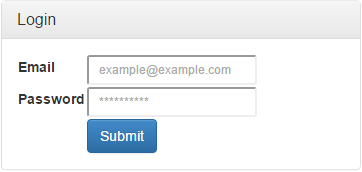
\includegraphics[width=0.5\textwidth]{img/zf2/login-container.png}
	\caption{Login container}
	\label{fig:login-container}
\end{figure}
	
	\subsection{Voucher system}

This system required operations with money and we come up with great solution, to implement voucher system. Customers have to buy vouchers to top up their balance on the account. Cards has to be printable and in order to do so I am generating a \textit{*.pdf} file that can be printed or saved for future printing. Voucher contains short information about company and \textit{QR code} that allow to scan by smartphone to simplify code inserting process. Figure \ref{fig:voucher} shows an example of printed voucher.

\begin{figure}[H]
	\centering
	
\includegraphics[width=0.5\textwidth]{img/zf2/voucher-example.png}
	\caption{Voucher example}
	\label{fig:voucher}
\end{figure}
	
To design this voucher and make it printable from web browser, I am using \textit{DOM pdf} generator. It allows to display remote pictures and specify fixed positions for text. \textit{QR Code} generating module submits the \textit{HTTP} request to Google API and receives a dynamic link to an image, which later in page generation I am using to add into \textit{pdf} file.


	\subsubsection{Lookup vouchers}
	

	\subsection{Order system}
		\subsubsection{Placed orders}
			When customer using their application places the order and transaction fully completed, then this order appears on the \textit{home page} as this system is designed to be pre order. At the certain time before collection system administrator prints out the list of food that has to be prepared for customer. In order to make a good printable layout it creates a \textit{*.pdf} file using \textit{JavaScript} module called PDF make ~\cite{PDF_Make_module}. It uses Document definition object and you do not have to calculate position manually as like in other pdf generation libraries. For example it can be as simple as:
			\\
			\begin{minted}{JavaScript}
var docDefinition = {
content: [
    // if you don't need styles, you can use a simple string to define a paragraph
    'This is a standard paragraph, using default style',

    // using a { text: '...' } object lets you set styling properties
    { text: 'This paragraph will have a bigger font', fontSize: 15 },

    // if you set pass an array instead of a string, you'll be able
    // to style any fragment individually
    {
      text: [
        'This paragraph is defined as an array of elements to make it possible to ',
        { text: 'restyle part of it and make it bigger ', fontSize: 15 },
        'than the rest.'
      ]
    }
  ]
};
			\end{minted}
			
			
			When you have prepared your document-definition-object, you can run the function that will parses it and generated \textit{pdf}:
			\\
			
			\begin{minted}{JavaScript}
// open the PDF in a new window
pdfMake.createPdf(docDefinition).open();
 
// print the PDF (temporarily Chrome-only)
pdfMake.createPdf(docDefinition).print();
 
// download the PDF (temporarily Chrome-only)
pdfMake.createPdf(docDefinition).download('optionalName.pdf');
			\end{minted}
			
			After order has been processed and collected, administrator has to go back to this system and mark collected orders. To simplify this process there is a check box beside each order and when all collected orders are marked user have to click \textit{Collected} button to make an update.
			\\
			In case of emergency some customer canceled their order administrator is allowed to cancel selected order and return money to customers account. In that case this order will not appear in later reports.
			
		\subsubsection{Order Reports}
			In order to make an accounting report in the orders tab, administrator can select two types of reports:
			\begin{itemize}
				\item \textbf{Daily report}
				\item \textbf{Periodic report}
			\end{itemize} 
			
			To view daily report user should specify the date in \textit{mm/dd/yyyy} format and press submit button as you can see in figuer \ref{fig:select-report-page}. 
			
			\begin{figure}[H]
				\centering
				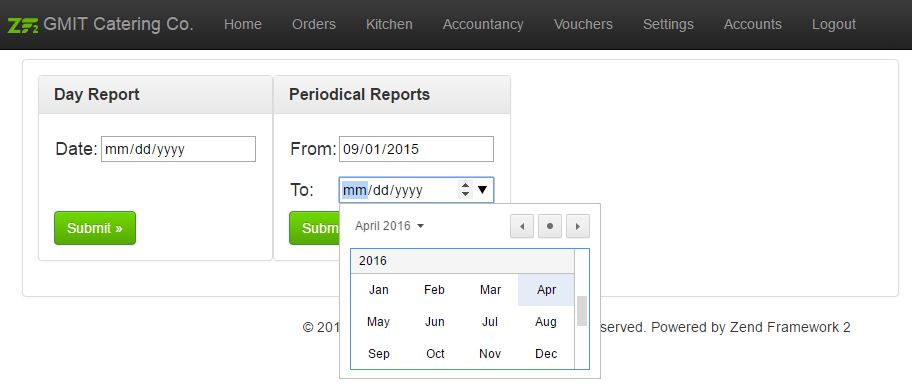
\includegraphics[width=1\textwidth]{img/zf2/01-canteen_select_periodic_report_page.png}
				\caption{Daily/Periodic report page}
				\label{fig:select-report-page}
			\end{figure}
			
			In the new page it will display report based on the period or specific date. Where user can go further and click order details, see customer's information or print this page as a report, see figure \ref{fig:daily-report-page}.
			
			\begin{figure}[H]
				\centering
				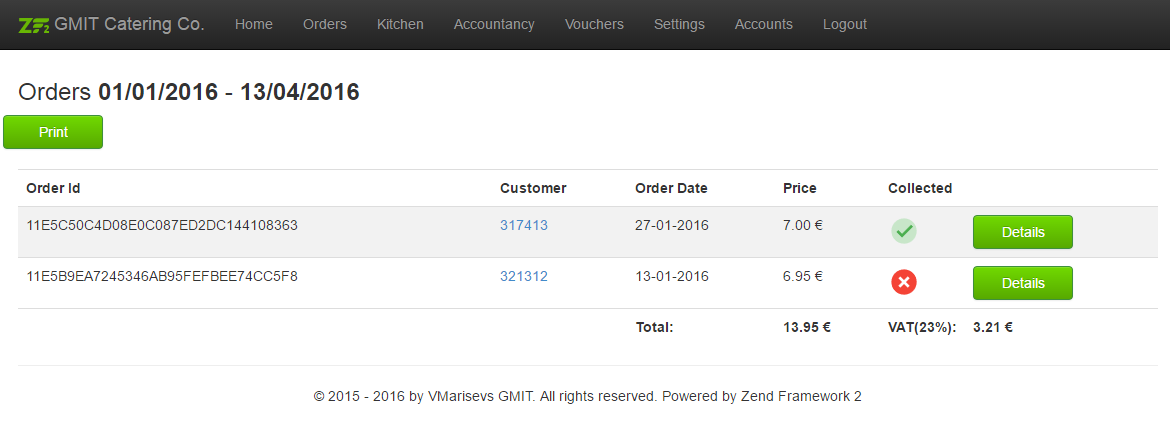
\includegraphics[width=1\textwidth]{img/zf2/01-canteen_select_periodic_report_page_1.png}
				\caption{Daily/Periodic report page}
				\label{fig:daily-report-page}
			\end{figure}
			
			Order details will display full information about customer and items ordered. It can be printed separately as invoice (see figure \ref{fig:order-invoice-page}) or proceed to go and view customer personal details.
			
			\begin{figure}[H]
				\centering
				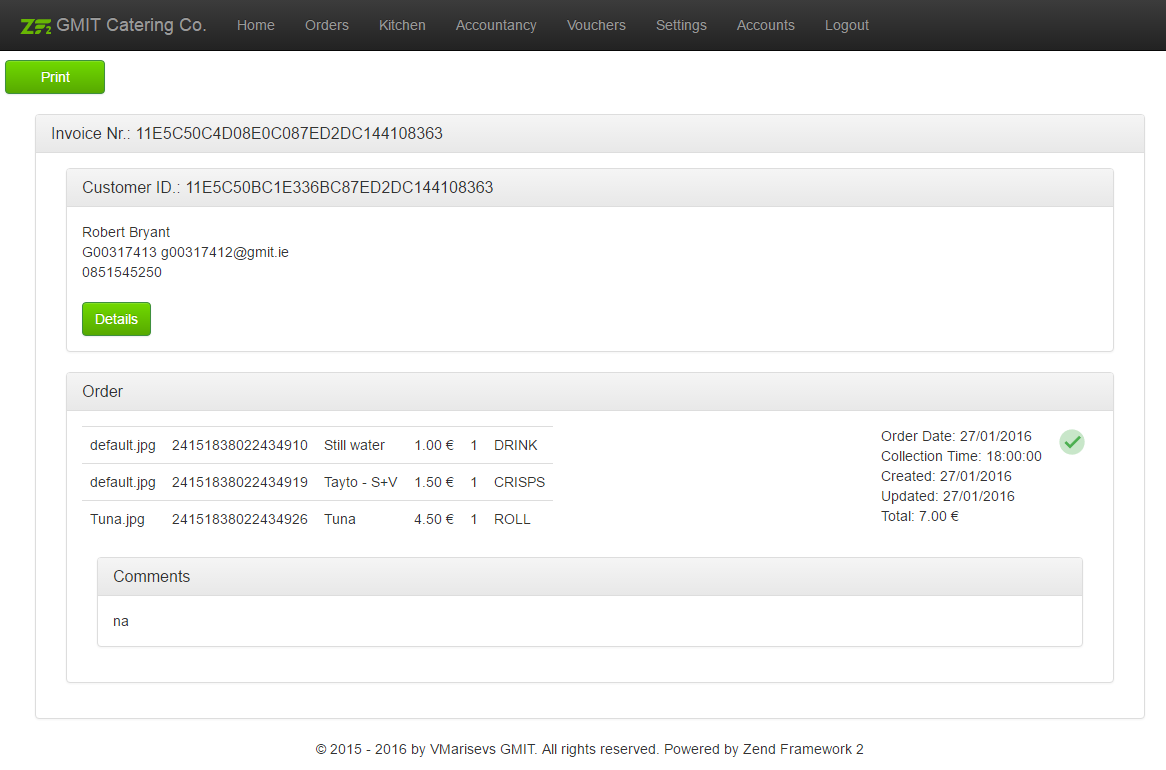
\includegraphics[width=1\textwidth]{img/zf2/01-canteen_select_periodic_report_page_2.png}
				\caption{Daily/Periodic report page}
				\label{fig:order-invoice-page}
			\end{figure}
			
			
		
		
		
	\subsection{Customer and accountancy}
		\subsubsection{Customer details}
		
		Authorized person can view all registered customers in accountancy tab and by clicking \textit{view} button. It will display a table with all users see in figure \ref{fig:customer-list}
		
		\begin{figure}[H]
			\centering
			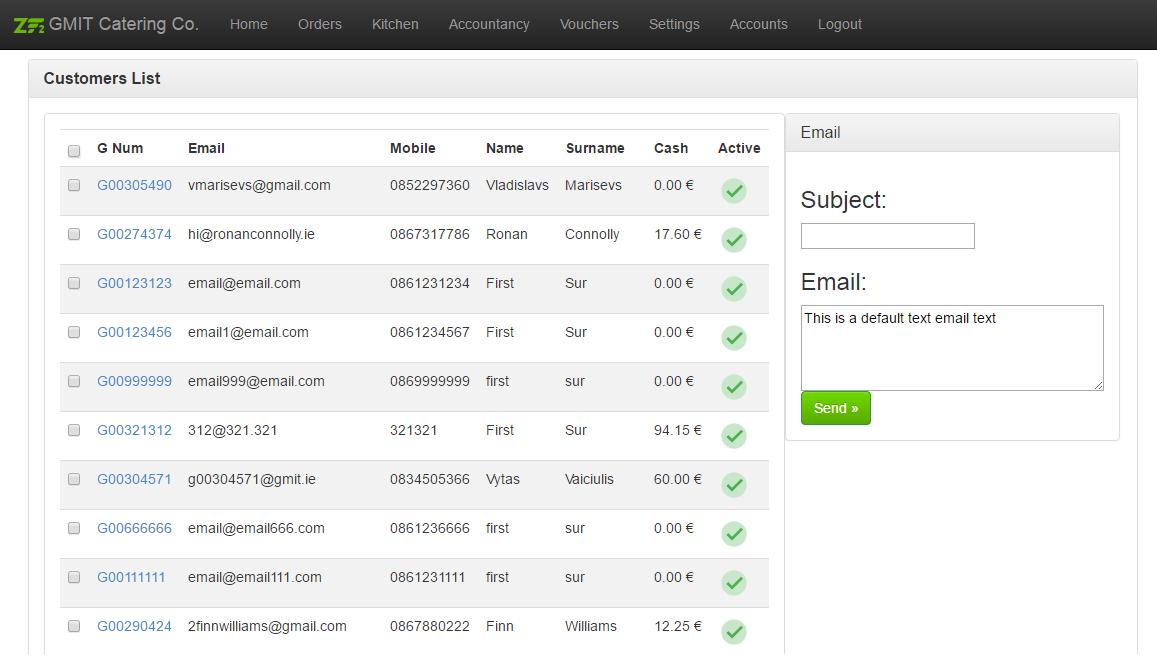
\includegraphics[width=1\textwidth]{img/zf2/04-customers.png}
			\caption{Customers list}
			\label{fig:customer-list}
		\end{figure}
		
		In this page we can select customers which we want to inform in updates and send them an email from default email. 
		% (This configuration was mentioned earlier in Database chapter)
		When person is found we can view his details as you can see in \ref{fig:customer-details} figure.
		
		\begin{figure}[H]
			\centering
			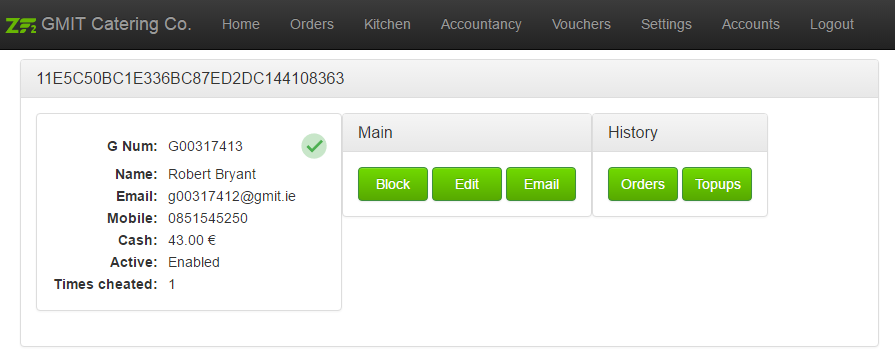
\includegraphics[width=1\textwidth]{img/zf2/02-customer_information.png}
			\caption{Customers details}
			\label{fig:customer-details}
		\end{figure}
		
		In this section we are able to do such things like send an email to customer, block him or edit his personal details in case they are wrong. We can determine that this cheated once, this counter increments only when person tries to enter wrong QR code as their voucher. 
		
		\subsubsection{Customer history}
		User has two types of histories. First one keeps a track of all user orders, so in future it can suggest user to make similar orders and history of user balance top up.
		
		
		\begin{figure}[H]
			\centering
			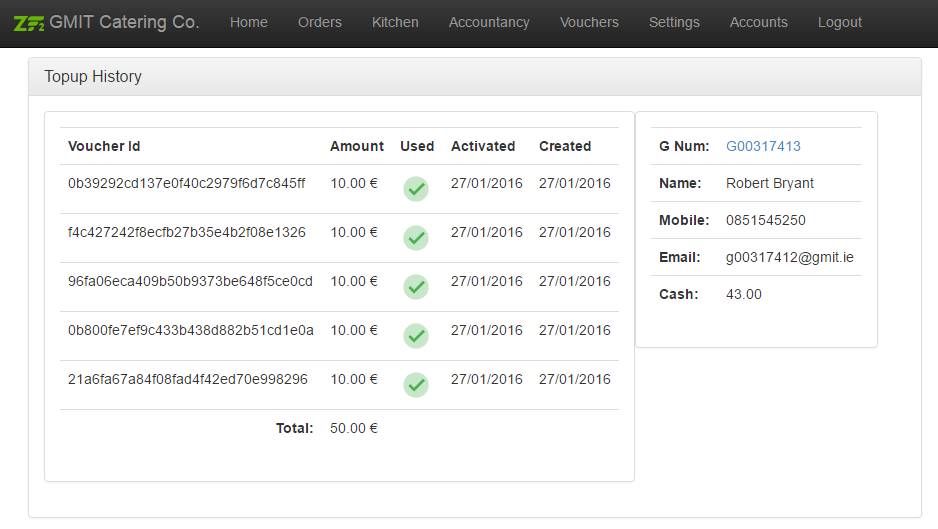
\includegraphics[width=1\textwidth]{img/zf2/02-customer_information_topup_history.png}
			\caption{Customers top up history}
			\label{fig:customer-topup-history}
		\end{figure}
		
		\begin{figure}[H]
			\centering
			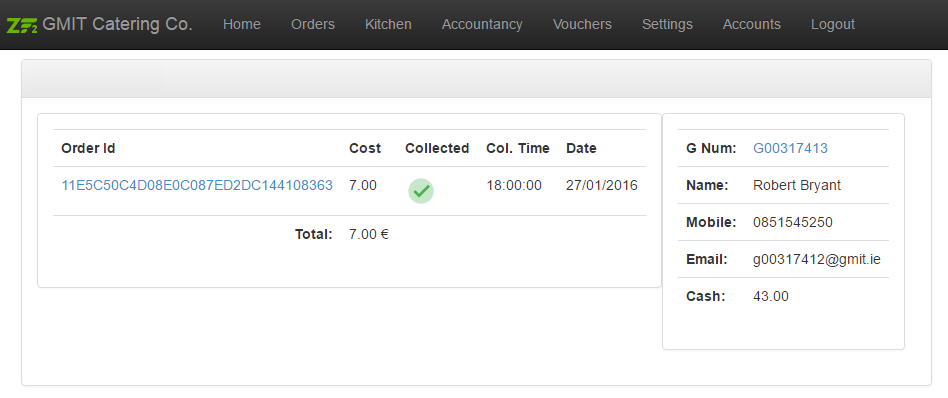
\includegraphics[width=1\textwidth]{img/zf2/02-customer_information_order_history.png}
			\caption{Customers order history}
			\label{fig:customer-order-history}
		\end{figure}
		
	\subsection{Ionic routes \& functions}
		\subsubsection{Authenticate customer}
		\subsubsection{Recover customers password}
		\subsubsection{Change customers password}
		\subsubsection{Sign Up new customer}
		\subsubsection{Top Up customer balance}
		\subsubsection{Approve customer's order and purchase}
		\subsubsection{Show customers history}
		\subsubsection{Show available food}
	
	

\subsection{PDF make}

~\cite{PDF_Make_module}



  \section{Mobile App}


\chapter{System Evaluation}	% n-m pages
\section{Web App}
	\subsection{PDF make vs DOM PDF}
		why???
	
\section{Mobile App}


\chapter{Conclusion}	% 1-3 pages

\begin{comment}
\begin{itemize}
\item Briefly summarise your context and ob-jectives (a few lines).
\item Highlight your findings from the evalua-tion section / chapter and any opportuni-ties identified.
\end{itemize}
\end{comment}
